\chapter{Preliminary work}
\label{chapter:pre_work}
In order to compute the metrics explained in the previous chapter, it is necessary to know the position and orientation (pose) of the contact points located on the phalanges of Vizzy.
\par

It is important to note that through the Denavit Hartenberg parameters and the angles of rotation of each joint it is possible to obtain the position and orientation of each sensor in 3D coordinates.

\par
It is known that the tactile sensors have incorporated sensors with Hall-effect that detects changes in the magnetic field caused, either by the magnet in the elastomer or by the Earth's magnetic field.
In the case where the sensors are not pressed, the influence of the magnetic field is constant, leaving only the Earth's magnetic field responsible for the change of the magnetic field of the sensor.

\par

The idea that came up was that, through the magnetic field readings, be able to discover the position and orientation of the phalanges. To test this idea, an experiment was carried out, in which it consists on obtaining data of the magnetic fields of each sensor placed in each phalanx and the angle of rotation between that same phalanx and the palm of the hand.
With these data, a relationship (through a regression) between each of the 3D components of the magnetic field from the sensor and its angle of rotation relative to the hand will be inferred.
\par

To obtain the ground-truth of the rotation angles, it was used \textit{Aruco} markers that were placed on each of the phalanges. \textbf{(visible in figure xxx).}
It is important to note that the first tests were performed with only one marker on each phalanx, which led to poses with a lot of uncertainties and in some cases the data did not make great sense. To correct these uncertainties were used markers boards ( 4 single markers in a column), which led to results with almost no uncertainty.

\par
These boards give their poses, which with the help of a function of ROS transformations it is obtained the angles of rotation between the board on the phalanx and the board on the anterior phalanx (towards the palm), this is done for each one phalanx of the index finger. These rotation angles will coincide with those of the joints.

\par

In the experiments that took place, the palm of Vizzy's hand was turned in the direction of the ground (i.e. the palm of the hand was parallel to the plane of the ground).
Then, starting from the point where the hand was open, Vizzy began to close his index finger to its final limit, later he opened his finger again until it was fully extended.
Finally, the data of the tactile sensors and the joint angles were analyzed.

In order to understand the graphics of the 3D components of the magnetic field as a function of the angles of rotation, the numbering of the finger sensors in \textbf{Figure xxx}.
\par
The graphics of the magnetic field components as a function of the angles of rotation are shown in Figures \ref{fig:1and2Joint} and \ref{fig:3Joint}. It is noted that there is only a direct relationship between the components of the sensors of each phalanx and the angle of rotation of its previous joint.

It is yet visible that there are components with more noise than others, such is the example of the Y component of the magnetic field of the Figures \ref{fig:2Joint_5sensor} and \ref{fig:3Joint_4sensor}.
It is important to note that in this report the equations of these graphics have not yet been defined because it is still necessary to remove the effect of the earth's magnetic field in relation to the orientation of the pulse.
To take this effect, will be placed an inertial sensor will be placed on the head of Vizzy. Moreover this work will be developed during the thesis.
\begin{figure}
\centering
\begin{subfigure}{.5\textwidth}
  \centering
  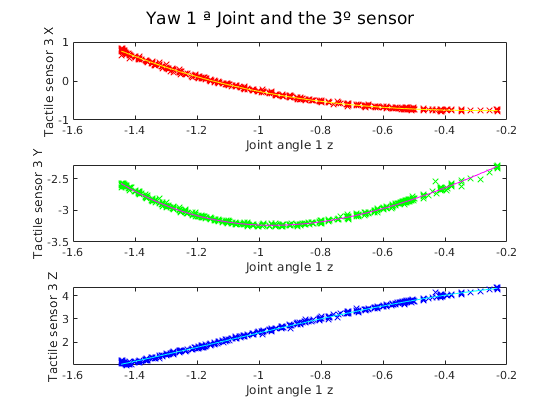
\includegraphics[width=1\linewidth]{images/1Joint_3sensor.png}
  \caption{\nth{1} Joint and the \nth{3} Tactile Sensor}
  \label{fig:fig:1Joint_3sensor}
\end{subfigure}%
\begin{subfigure}{.5\textwidth}
  \centering
  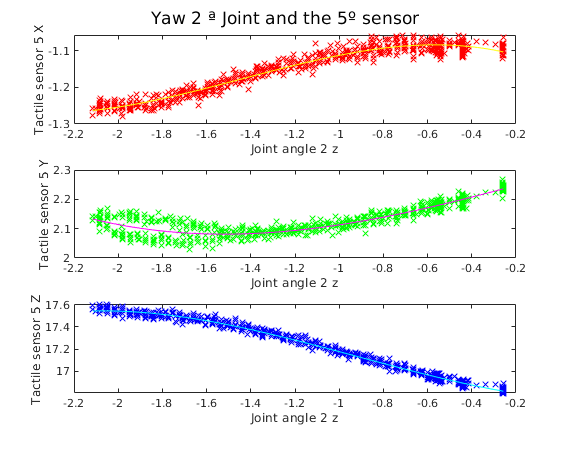
\includegraphics[width=1\linewidth]{images/2Joint_5sensor.png}
  \caption{\nth{2} Joint and the \nth{5} Tactile Sensor}
  \label{fig:2Joint_5sensor}
\end{subfigure}
\caption{Graphics of the magnetic field components as a function of the \nth{1} and \nth{2} rotation angles }
\label{fig:1and2Joint}
\end{figure}

\begin{figure}
\centering
\begin{subfigure}{.5\textwidth}
  \centering
  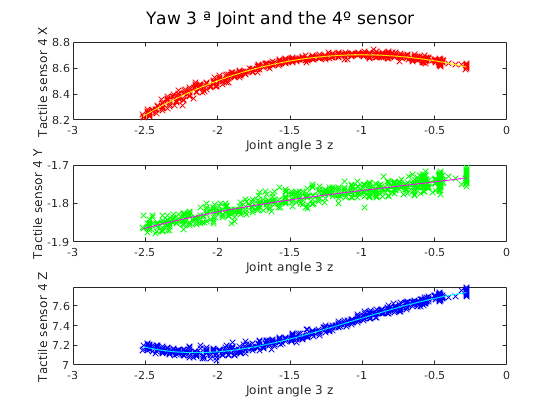
\includegraphics[width=1\linewidth]{images/3Joint_4sensor.png}
  \caption{\nth{3} Joint and the \nth{4} Tactile Sensor}
  \label{fig:3Joint_4sensor}
\end{subfigure}%
\begin{subfigure}{.5\textwidth}
  \centering
  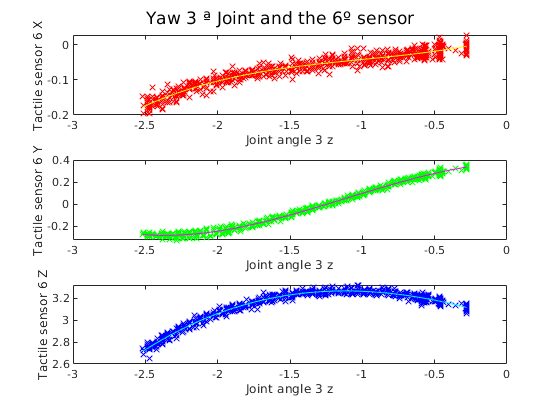
\includegraphics[width=1\linewidth]{images/3Joint_6sensor.png}
  \caption{\nth{3} Joint and the \nth{6} Tactile Sensor}
  \label{fig:3Joint_6sensor}
\end{subfigure}
\caption{Graphics of the magnetic field components as a function of the \nth{3} rotation angle }
\label{fig:3Joint}
\end{figure}

